\section{Gathering performance metrics}
\label{sec:performance}
Although the system is very flexible and allows replication of components, it does not contain any component that is able to evaluate it's state and make decisions regarding allocation and release of resources, consequently scaling must be done manually. Manual scaling the system can become a complex problem because each component has different resource requirements and even the same component can use more or less of a resource, depending on the job that it must execute. Monitoring the system manually and scaling it quickly become unmanageable and an automated way to do the scaling is desirable. 

In order to scale the system automatically, key performance metrics must be gathered and analysed. Some of the basic performance parameters that can be gathered for a component are CPU, memory and network usage. Knowing the resource utilization of one component allows us to take decisions regarding deployment of that component. For example we can have 2 component, one with high CPU usage and one with high network usage, it would be efficient to collocate replicas of those components on the same VM or to allocate the ones that require high CPU usage to VM's with more computing power. By having this insight on component resource utilization we are able to take those decisions and use the resources  we have in an efficient way. But resource utilization for components can vary with time, so a static scheme is not very useful, because it becomes outdated in a short period of time. Continuous monitoring the components and taking actions on fresh performance metrics is crucial in guaranteeing optimal allocation strategies.

\subsection{Monitoring CPU}
A first step would be to monitor the CPU usage in order to find a rough approximation of how much computing power does a component need. The main challenge here is to find tools that are able to monitor short lived processed, under 1 second, and to report with high accuracy the CPU usage in order to take decisions for component allocation. Four tools/methods for gathering CPU usage statistics were reviewed:  
\begin{itemize}
	\item "ManagementFactory" is a class from the Java standard library that is able to collect performance metrics from the JVM. The main drawback is that Nma\footnote{https://nmap.org}, one of the tools used by the system we want to extend, is an external program and it cannot be monitored by this library.
	\item "Sigar"\footnote{https://github.com/hyperic/sigar} library for Java can be used to monitor arbitrary process identifiers (PIDs), but the problem is that we first have to start the component, obtain its PID and only after we can start monitoring it with "Sigar" library, the main problem is that we might lose the CPU usage at the start of the process which can be introduce high error rates in the allocation phase.
	\item "pidstat" and "top" tools have the same drawbacks. they miss the CPU usage for the process if it is very short lived and the CPU usage of the process right before it ends, but they are better alternatives than the tools mentioned before because they can monitor processes from the moment they are crated, not missing the CPU usage from the start of the process.
	\item "atop" tool can monitor processes from the moment they are crated and capture the CPU usage of the process right before it terminates. Because it is able to capture the CPU usage at the start and at the end of the lifetime of a process, it provides very accurate results introducing small overhead on the system. The only drawback that was found is related to the root privileges that are needed in order to run this tool.
\end{itemize}
 
\begin{figure}[t]
\centering
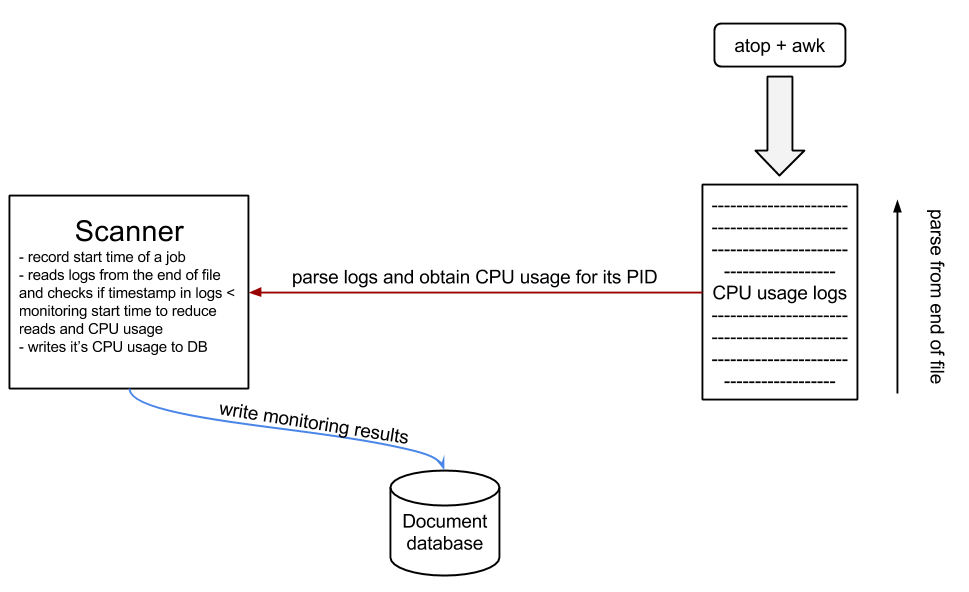
\includegraphics[width=\linewidth]{./img/MonitoringCPUMechanism.png}
\caption{Distributed performance monitoring system architecture}
\label{fig:monitoringArchitecture}
\end{figure} 
 
The tool "atop" was chosen to measure CPU usage because of it's high accuracy and low overhead. In the first implementation "atop" was called at the begging of each new job for each component, but this approach had some problems because it took some time to start "atop" and CPU usage was not recorded for the start of the process. This approach  required launching "atop" for each job and for each component making it consume considerable system resources. 

The second approach was to launch "atop" from an external script, parse it's results and store them in a log file. The second approach was much better because it allowed using only one "atop" instance to gather CPU usage statistics for all running processes on a system, and each component that was interested in it's CPU usage could have just parsed the log file. Another advantage was that it decoupled the monitoring activities from the components that were monitored. The architecture for the second approach is presented in Fig. \ref{fig:monitoringArchitecture}, the log document is read from the bottom upwards, because the chances are that the monitoring results will be closer to the bottom than to the top.

Fig. \ref{fig:monitoringArchitectureExtended}  presents an architecture that is even more decoupled than the one presented in Fig. \ref{fig:monitoringArchitecture}, the parsing is done in a different component "Monitor" and the components only need to save the beginning and the end time for a job they executed, the parsing of the monitoring data would be done by the "Monitor" component. This architecture ads more flexibility, because the "Monitor" component can be on the same machine to minimize network traffic,  or on a different machine in order to minimize computational costs on the machines that is being monitored. Using this approach we can use the monitoring system independently of the target we are monitoring, allowing us to separate the monitoring concern from the logic that is implemented in the tools that we are monitoring.


\begin{figure}
\centering
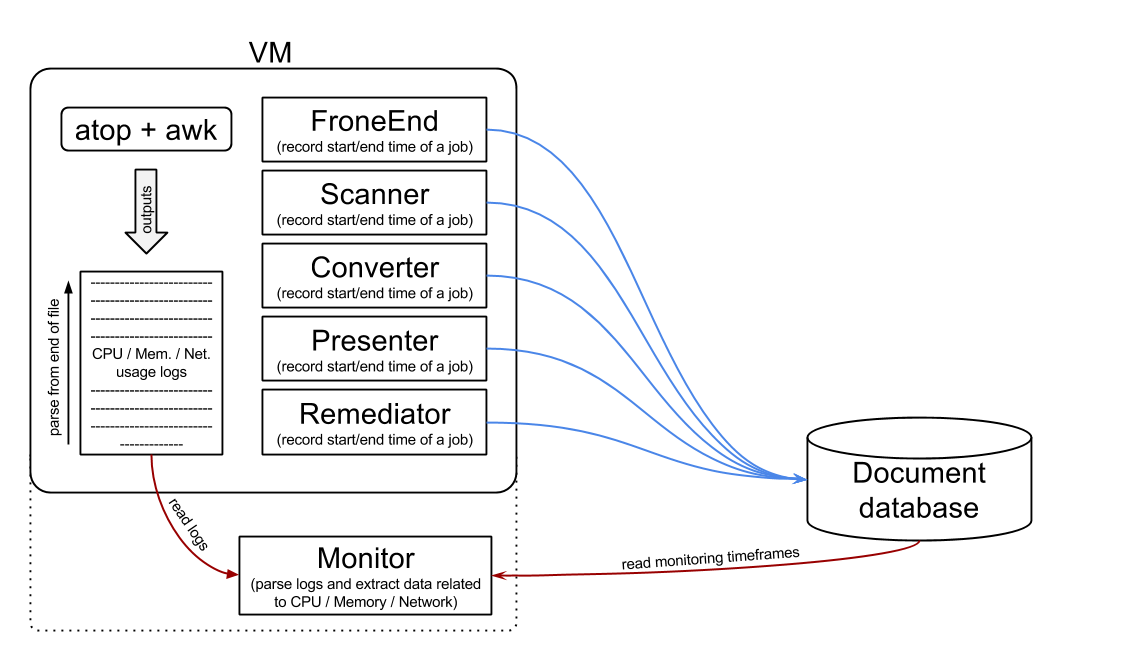
\includegraphics[width=\linewidth]{./img/MonitoringCPUMechanismExtended.png}
\caption{Distributed performance monitoring system architecture}
\label{fig:monitoringArchitectureExtended}
\end{figure}
